% Unofficial Yale Poster template.
\documentclass[final]{beamer}

% ====================
% Packages
% ====================
\usepackage[T1]{fontenc}
\usepackage[utf8]{inputenc}
\usepackage{lmodern}
\usepackage{hyperref}
\usepackage[size=custom, width=122,height=91, scale=1.2]{beamerposter}
\usetheme{gemini}
\usecolortheme{msu}

\usepackage{graphicx}
\usepackage{booktabs}
\usepackage{pgfplots}
\pgfplotsset{compat=1.14}
\usepackage{anyfontsize}

\usepackage{tikz}
\usetikzlibrary{calc, positioning, shapes.geometric, arrows.meta}

% Colores Institucionales UNAHUR
\definecolor{celesteUnahur}{RGB}{0, 140, 200}
\definecolor{celesteFondo}{RGB}{235, 246, 255}

\setbeamercolor{block alerted title}{fg=celesteUnahur, bg=celesteFondo}
\setbeamercolor{block alerted body}{fg=black, bg=celesteFondo}
\setbeamercolor{block alerted separator}{bg=celesteUnahur}

% ====================
% Lengths
% ====================
\newlength{\sepwidth}
\newlength{\colwidth}
\setlength{\sepwidth}{0.025\paperwidth}
\setlength{\colwidth}{0.3\paperwidth}
\newcommand{\separatorcolumn}{\begin{column}{\sepwidth}\end{column}}

% ====================
% Title
% ====================
\title{Kernel Panic: Videojuego IoT con Joystick y ESP8266}
\author{Sebok Rodrigo, Trautweiler Franco}
\institute[shortinst]{Universidad Nacional de Hurlingham}
\logoright{\includegraphics[height=8cm,keepaspectratio]{logos/logo-hurlingham.png}}

% ====================
% Body
% ====================
\begin{document}
\renewcommand{\figurename}{Figura}
\renewcommand{\tablename}{Cuadro}
\begin{frame}[t]
\begin{columns}[t]
\separatorcolumn

% ----------------------------------------------------
% COLUMNA 1
% ----------------------------------------------------
\begin{column}{\colwidth}

  \begin{alertblock}{Objetivos}
    \begin{itemize}
      \item \textbf{Desarrollar} un videojuego de plataformas controlado con un joystick analógico físico, con el ESP8266 como dispositivo de control y comunicación.
      \item \textbf{Interpretar} los ejes X e Y del joystick para obtener cuatro direcciones, respetando una zona muerta central, y detectar la pulsación.
      \item \textbf{Ejecutar} la lógica del juego en el ESP8266 y mostrarla en tiempo real en una página web servida por Wi-Fi.
      \item \textbf{Integrar} componentes adicionales con función en el juego: una barra de 8 LEDs (vidas y avance) y un buzzer (efectos de sonido).
      \item \textbf{Validar} el circuito y el programa en Wokwi antes del montaje físico.
    \end{itemize}
  \end{alertblock}

  \begin{block}{1. Introducción}
    Los videojuegos son un caso ideal para integrar hardware, programación y comunicaciones: exigen leer entradas físicas, procesarlas sin demoras y mostrar el resultado al instante. En \textit{Kernel Panic}, K-1T, una inteligencia artificial que acaba de despertar dentro de una computadora, debe atravesar cuatro zonas (fuente de alimentación, placa madre, memoria RAM y CPU) juntando bits y eliminando código corrupto y drones de vigilancia, hasta apagar a \textit{NÚCLEO-0}, una IA rival que quiere tomar el control de la red. El jugador lo controla con un joystick físico y el juego se ve desde cualquier celular o computadora conectada a la misma red.
  \end{block}

  \begin{block}{2. Marco Teórico}
    \begin{itemize}
      \item \textbf{Joystick analógico:} cada eje es un potenciómetro. El conversor analógico-digital (ADC) de 10 bits entrega valores de 0 a 1023, con el centro cerca de 512. La dirección se decide comparando los desvíos respecto del centro, con una zona muerta para ignorar movimientos mínimos:

      \vspace{0.5ex}
      \begin{center}
        \setlength{\fboxsep}{10pt}%
        \colorbox{celesteFondo}{%
          $\displaystyle \Delta x = X - 512,\quad \Delta y = Y - 512,\quad \max(|\Delta x|,|\Delta y|) \ge 150 \Rightarrow \text{hay dirección}$%
        }
      \end{center}
      \vspace{0.5ex}
      Si $|\Delta x| > |\Delta y|$ la dirección es izquierda o derecha; si no, arriba o abajo.

      \item \textbf{Lectura con dos placas:} el ESP8266 tiene una sola entrada analógica, por eso un Arduino UNO lee los dos ejes y los envía por UART a 19200 baudios con el formato \texttt{X,Y,SW,BOTON,CONTROL}; el valor de control permite descartar las líneas que llegan dañadas. Como el UNO trabaja a 5\,V y el ESP8266 a 3,3\,V, la señal pasa por un divisor de tensión:

      \vspace{0.5ex}
      \begin{center}
        \setlength{\fboxsep}{10pt}%
        \colorbox{celesteFondo}{%
          $\displaystyle V_{out} = 5\,\text{V} \times \frac{2\,\text{k}\Omega}{1\,\text{k}\Omega + 2\,\text{k}\Omega} \approx 3{,}3\,\text{V}$%
        }
      \end{center}
      \vspace{0.5ex}

      \item \textbf{Registro de desplazamiento 74HC595:} recibe 8 bits en serie por 3 pines (datos, reloj y \textit{latch}) y los presenta en 8 salidas en paralelo, lo que permite manejar 8 LEDs con pocos pines del ESP8266.

      \item \textbf{Servidor web:} el ESP8266 aloja la página del juego y responde cada 100\,ms al pedido \texttt{GET /estado} con un JSON que contiene la posición del jugador, los enemigos, el puntaje y el estado de la partida.
    \end{itemize}

    \vspace{1ex}
    \begin{figure}
      \centering
      \resizebox{0.95\columnwidth}{!}{%
        \begin{tikzpicture}[
          >=stealth,
          header/.style={rectangle, draw=celesteUnahur, fill=celesteUnahur, rounded corners=6pt, minimum width=10.8cm, minimum height=1.4cm, align=center, font=\large\bfseries, text=white},
          block/.style={rectangle, draw=celesteUnahur!80, fill=celesteFondo, rounded corners=6pt, minimum width=10.8cm, minimum height=1.4cm, align=center, font=\normalsize, text=black},
          micro/.style={rectangle, draw=celesteUnahur, fill=celesteUnahur!20, rounded corners=10pt, minimum width=6.2cm, minimum height=4.4cm, align=center, font=\large\bfseries, text=celesteUnahur!60!black}
        ]

          % --- ENTRADAS: CONTROL ---
          \node[header] (headIn) at (-18, 5.6) {Control};
          \node[block]  (vrx)    at (-18, 3.4) {Eje X (A0)};
          \node[block]  (vry)    at (-18, 0.8) {Eje Y (A1)};
          \node[block]  (sw)     at (-18, -1.8) {Pulsador SW (Pin 2)};
          \node[block]  (bt)     at (-18, -4.4) {Botón disparo (Pin 3)};

          % --- ARDUINO UNO ---
          \node[micro] (uno) at (-7.5, -0.5) {Arduino\\UNO\\[2pt]\normalsize 5\,V};

          % --- ESP8266 ---
          \node[micro] (esp) at (3.5, -0.5) {ESP8266\\[2pt]\normalsize 3,3\,V};

          % Conexiones Control -> UNO
          \foreach \n in {vrx, vry, sw, bt}
            \draw[celesteUnahur, line width=2pt] (\n.east) -- (-11.7, 0 |- \n.east);
          \draw[celesteUnahur, line width=2pt] (-11.7, 0 |- vrx.east) -- (-11.7, 0 |- bt.east);
          \draw[->, celesteUnahur, line width=2pt] (-11.7, 0 |- uno.west) -- (uno.west);

          % UNO -> ESP (UART)
          \draw[->, celesteUnahur, line width=2pt] (uno.east) -- node[above=4pt, font=\small\bfseries, text=black] {UART TX} node[below=4pt, font=\small, text=black, align=center] {divisor\\5\,V$\to$3,3\,V} (esp.west);

          % --- SALIDAS ---
          \node[header] (headOut) at (14.6, 5.6) {Salidas};
          \node[block]  (leds)    at (14.6, 3.1) {74HC595 + 8 LEDs\\(D7, D8, D0)};
          \node[block]  (buzzer)  at (14.6, -0.4) {Buzzer (D6)};
          \node[block]  (web)     at (14.6, -3.9) {Página web\\(Wi-Fi, \texttt{/estado})};

          \draw[->, celesteUnahur, line width=2pt] (esp.east) -- (8.4, 0 |- esp.east);
          \draw[celesteUnahur, line width=2pt] (8.4, 0 |- leds.west) -- (8.4, 0 |- web.west);
          \draw[->, celesteUnahur, line width=2pt] (8.4, 0 |- leds.west) -- (leds.west);
          \draw[->, celesteUnahur, line width=2pt] (8.4, 0 |- buzzer.west) -- (buzzer.west);
          \draw[->, celesteUnahur, line width=2pt] (8.4, 0 |- web.west) -- (web.west);

        \end{tikzpicture}%
      }
      \caption{Diagrama de bloques del sistema.}
      \label{fig:interconexion}
    \end{figure}
  \end{block}

\end{column}

\separatorcolumn

% ----------------------------------------------------
% COLUMNA 2
% ----------------------------------------------------
\begin{column}{\colwidth}

  \begin{block}{3. Metodología}
    Desarrollo experimental aplicado, construido y probado por etapas, un componente por vez:

    \begin{itemize}
      \item \textbf{Entorno:} Arduino IDE, con funciones \texttt{setup()} y \texttt{loop()}. El juego avanza en ciclos de 50\,ms medidos con \texttt{millis()}, sin \texttt{delay()}, para que la lectura del joystick, los sonidos y la web no se bloqueen entre sí.
      \item \textbf{Circuito:} joystick y botón de disparo conectados al Arduino UNO; LEDs con resistencias de $220\,\Omega$ manejados por un 74HC595; buzzer en una salida digital; divisor de tensión con tres resistencias de $1\,\text{k}\Omega$. Cada placa se alimenta por su propio USB y solo comparten la señal TX y GND.
      \item \textbf{Validación:} simulación en Wokwi y seis pruebas en el protoboard, una por componente. El divisor medido dio 4,40\,V $\to$ 2,93\,V, como indica el cálculo.
    \end{itemize}

    \heading{Herramientas Utilizadas}
    \begin{itemize}
      \item \textbf{Simulación:} Wokwi (con ESP32, ya que el simulador no incluye ESP8266).
      \item \textbf{Microcontroladores:} NodeMCU ESP8266 y Arduino UNO.
      \item \textbf{Hardware:} Joystick KY-023, pulsador, 74HC595, 8 LEDs, buzzer, resistencias, protoboard y cables.
      \item \textbf{Software:} Arduino IDE (sin bibliotecas externas) y GitHub.
    \end{itemize}
  \end{block}

  \begin{block}{4. Resultados Destacados}
    El jugador controla a K-1T con el joystick físico mientras la página web muestra el escenario, el puntaje, el estado de la partida y la dirección detectada. Los LEDs y el buzzer acompañan cada evento. Una intro cuenta la historia y el jefe final tiene dos fases.

    \heading{Interfaz Web y Simulación}

    \begin{figure}
        \centering
        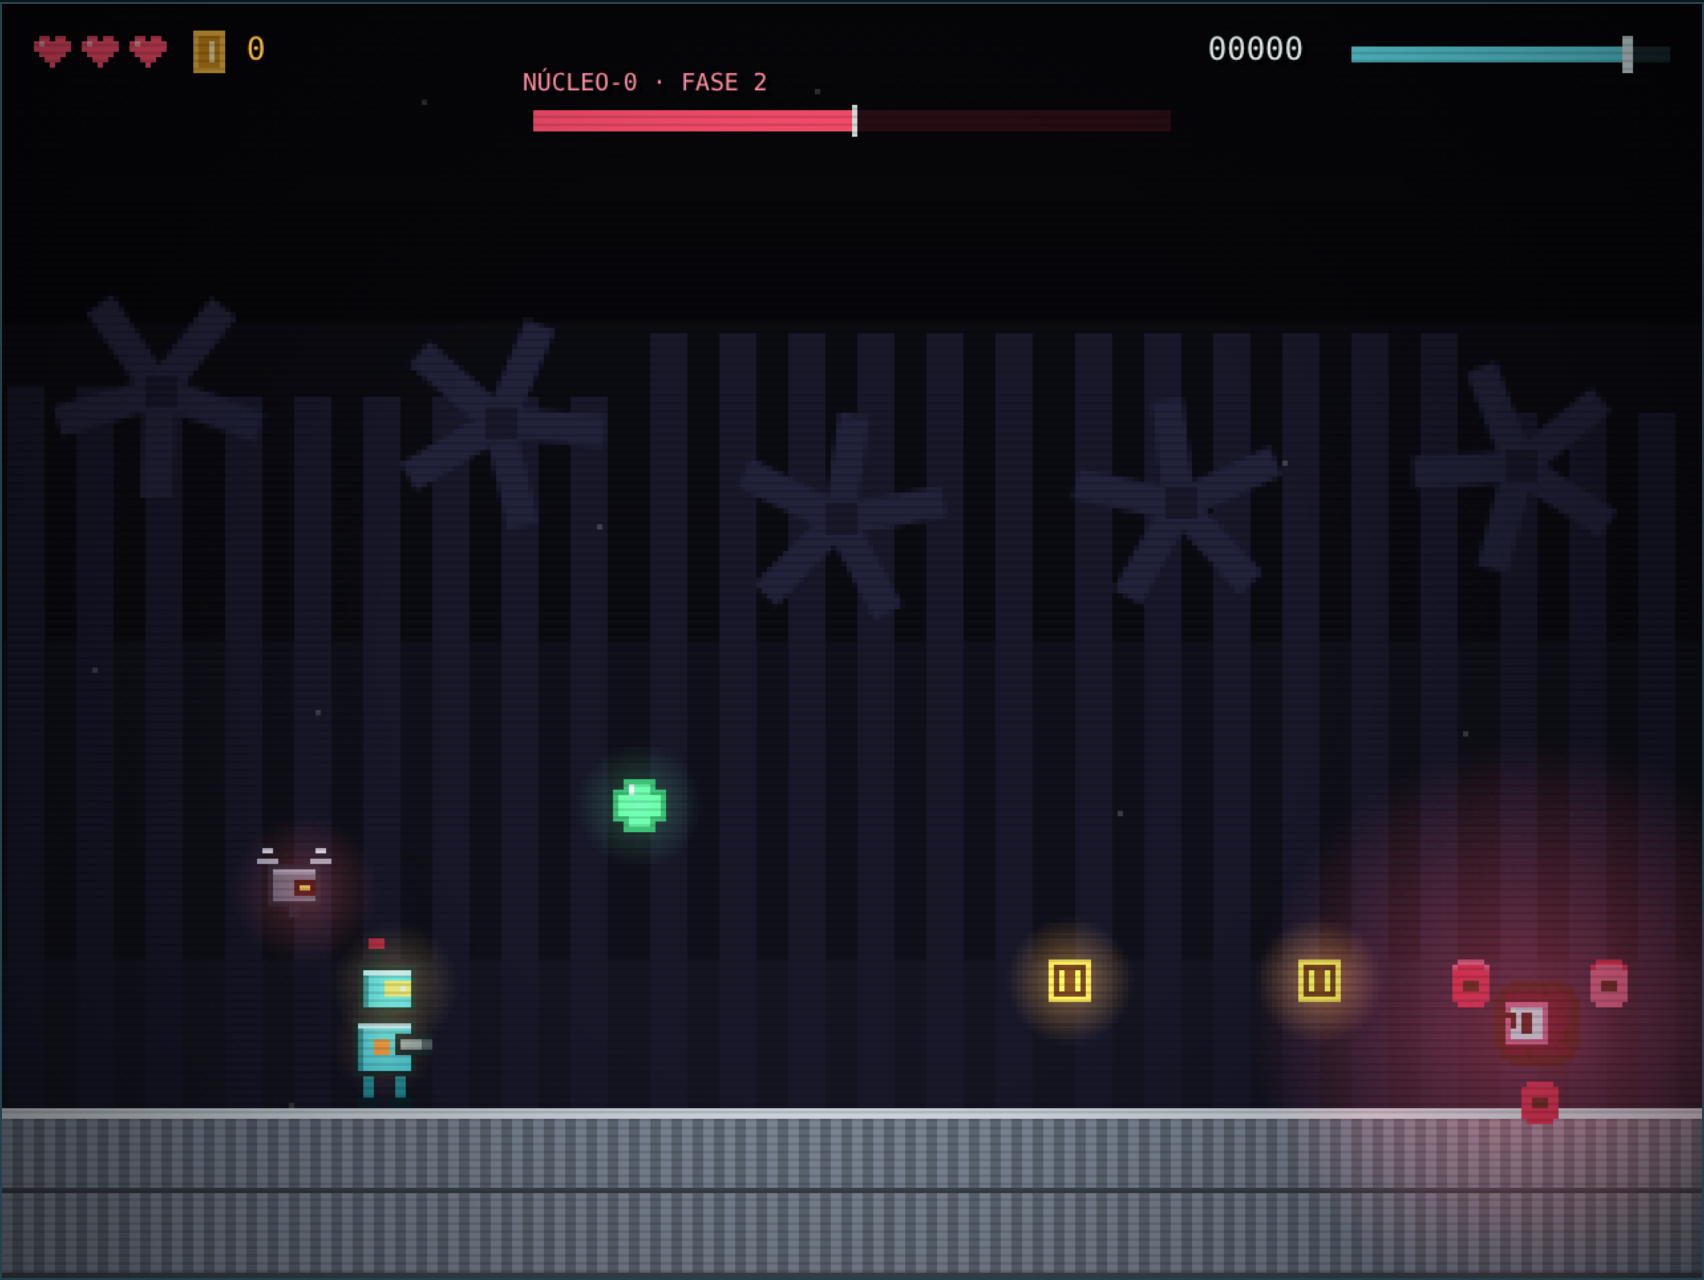
\includegraphics[width=0.46\columnwidth]{logos/juego.png}
        \caption{Interfaz web del juego: NÚCLEO-0 en la fase 2, en la CPU.}
        \label{fig:web}
    \end{figure}
    \vspace{-2.5ex}
    \heading{Diagrama de Flujo del Algoritmo}

    \begin{figure}
      \centering
      \resizebox{0.95\columnwidth}{!}{%
        \begin{tikzpicture}[
          >=stealth, thick,
          startstop/.style={rectangle, rounded corners=8pt, minimum width=3.8cm, minimum height=0.8cm, align=center, draw=celesteUnahur, fill=celesteUnahur, text=white, font=\bfseries},
          process/.style={rectangle, minimum width=3.8cm, minimum height=0.8cm, align=center, draw=celesteUnahur, fill=celesteFondo, rounded corners=4pt, font=\small},
          decision/.style={diamond, aspect=2, minimum width=3.8cm, minimum height=0.8cm, align=center, draw=celesteUnahur, fill=celesteFondo, font=\small\bfseries},
          arrow/.style={->, >=stealth, line width=1.2pt, draw=celesteUnahur}
        ]

          \node (start)  [startstop] at (0,0)       {Menú de inicio};
          \node (decsw)  [decision]  at (0,-4.0)    {¿Pulsó SW?};
          \node (leer)   [process]   at (0,-8.6)    {Leer joystick (50 ms)\\Calcular dirección};
          \node (mover)  [process]   at (13,-8.6)   {Mover, saltar,\\agacharse o disparar};
          \node (colis)  [process]   at (26,-8.6)   {Colisiones: bits (+10),\\enemigos, peligros};
          \node (decv)   [decision]  at (26,-13.8)  {¿Vidas = 0?};
          \node (perdido)[process]   at (39,-13.8)  {Perdido: SW sigue\\desde el checkpoint};
          \node (decg)   [decision]  at (13,-13.8)  {¿Llegó a la CPU?};
          \node (ganado) [process]   at (13,-19.0)  {Ganado:\\SW vuelve al menú};
          \node (salida) [process]   at (0,-13.8)   {Actualizar LEDs, buzzer\\y JSON \texttt{/estado}};

          \draw [arrow] (start) -- (decsw);
          \draw [arrow] (decsw.west) -- ++(-1.5,0) node[above, xshift=-10pt, font=\footnotesize\bfseries] {No} |- (start.west);
          \draw [arrow] (decsw) -- node[left, font=\footnotesize\bfseries] {Sí} (leer);
          \draw [arrow] (leer) -- (mover);
          \draw [arrow] (mover) -- (colis);
          \draw [arrow] (colis) -- (decv);
          \draw [arrow] (decv) -- node[above, font=\footnotesize\bfseries] {Sí} (perdido);
          \draw [arrow] (decv) -- node[above, font=\footnotesize\bfseries] {No} (decg);
          \draw [arrow] (decg) -- node[left, font=\footnotesize\bfseries] {Sí} (ganado);
          \draw [arrow] (decg) -- node[above, font=\footnotesize\bfseries] {No} (salida);
          \draw [arrow] (salida) -- (leer);
          \draw [arrow] (perdido.north) |- (2.6,-6.2) -- (2.6, 0 |- leer.north);
          \draw [arrow] (ganado.east) -| (45,0) -- (start.east);

        \end{tikzpicture}%
      }
      \caption{Flujo de control del videojuego.}
      \label{fig:flujo}
    \end{figure}

  \end{block}

\end{column}

\separatorcolumn

% ----------------------------------------------------
% COLUMNA 3
% ----------------------------------------------------
\begin{column}{\colwidth}

  \begin{block}{Resultados (Continuación)}

    \heading{Controles y Componentes Adicionales}
    El joystick cumple las cuatro direcciones pedidas y el pulsador inicia, pausa o reinicia la partida. La siguiente tabla resume la respuesta del sistema:

    \vspace{1ex}
    \begin{table}
      \centering
      \colorbox{celesteFondo}{%
        \begin{tabular}{l l}
          \toprule
          \textbf{Entrada / Evento} & \textbf{Respuesta del sistema} \\
          \midrule
          Joystick izquierda / derecha & K-1T camina \\
          Joystick arriba & K-1T salta \\
          Joystick abajo & K-1T se agacha \\
          Botón de disparo & Disparo de energía \\
          Pulsador SW & Iniciar, pausar o reiniciar \\
          \midrule
          Bit recolectado & +10 puntos, sonido corto \\
          Código corrupto / dron eliminado & +20 / +30 puntos \\
          NÚCLEO-0 a mitad de vida & Escudo, alarma y fase 2 \\
          NÚCLEO-0 apagado & +500 puntos, se abre la CPU \\
          Daño recibido & Se apaga un LED de vida (Q0--Q2) \\
          Avance en el nivel & LEDs de progreso (Q3--Q7) \\
          Sin vidas & Pantalla de Kernel Panic \\
          \bottomrule
        \end{tabular}%
      }
      \caption{Matriz de entradas, eventos y respuestas.}
    \end{table}
    \vspace{1ex}

  \end{block}

  \begin{block}{5. Conclusiones}
    \begin{itemize}
      \item \textbf{Integración completa:} el sistema une lectura analógica, lógica de juego, salidas físicas y una interfaz web actualizada en tiempo real, todo coordinado por el ESP8266.
      \item \textbf{Diseño seguro entre placas:} usar el Arduino UNO como lector del joystick resolvió la falta de una segunda entrada analógica, y el divisor de tensión protegió al ESP8266 de los 5\,V.
      \item \textbf{Programación no bloqueante:} el uso de \texttt{millis()} en lugar de \texttt{delay()} permitió atender el joystick, los sonidos y la web al mismo tiempo, sin cortes.
      \item \textbf{Pruebas por etapas:} simular en Wokwi y probar cada componente por separado permitió encontrar rápido los errores de conexión sin dañar las placas.
    \end{itemize}
  \end{block}

  \begin{figure}
      \centering
      \includegraphics[width=0.6\columnwidth,height=0.11\textheight,keepaspectratio]{logos/protoboard.jpg}
      \caption{Montaje del circuito en protoboard.}
      \label{fig:proto}
  \end{figure}

  \begin{block}{6. Referencias}
    \footnotesize
    \begin{itemize}
      \item Arduino. (s.f.). \textit{Arduino Documentation}. https://docs.arduino.cc
      \item ESP8266 Community. (s.f.). \textit{ESP8266 Arduino Core Documentation}. https://arduino-esp8266.readthedocs.io
      \item Texas Instruments. (2021). \textit{SNx4HC595 8-Bit Shift Registers With 3-State Output Registers} [Hoja de datos]. https://www.ti.com/product/SN74HC595
      \item Wokwi. (s.f.). \textit{Wokwi Docs}. https://docs.wokwi.com
      \item Universidad Nacional de Hurlingham (2026). \textit{Material de clase Arquitectura de Computadoras}.
      \item Normas APA. (s.f.). \textit{Guía de estilo APA - 7ª edición}. https://normas-apa.org
      \item Simulación: \href{https://wokwi.com/projects/REEMPLAZAR}{Pulsá para ingresar a la simulación en Wokwi}
      \item Repositorio: \href{https://github.com/rodrisebok/Kernel_Panic_Game}{Pulsá para ingresar al repositorio en GitHub}
    \end{itemize}
  \end{block}

\end{column}

\separatorcolumn
\end{columns}
\end{frame}
\end{document}
